
%(BEGIN_QUESTION)
% Copyright 2009, Tony R. Kuphaldt, released under the Creative Commons Attribution License (v 1.0)
% This means you may do almost anything with this work of mine, so long as you give me proper credit

Examine this loop diagram, and answer the following questions:

$$\includegraphics[width=15.5cm]{i0009rx01.eps}$$

\begin{itemize}
\item{} What type of control loop is represented in this diagram?  In other words, what is the process variable, and how is this process variable manipulated?
\vskip 10pt
\item{} What is the calibrated range of the sensing instrument?
\vskip 10pt
\item{} How are physical locations for wire connection points declared in this diagram?
\vskip 10pt
\item{} Assuming each of the two resistors in the circuit are 250 ohms, calculate the amount of voltage between terminals 23 and 24 at a transmitter signal value of 50\%.
\vskip 10pt
\item{} Identify where wires are part of a larger, multi-conductor cable, and identify how those wires are distinguished from all the others in that cable.
\vskip 10pt
\item{} Identify the convention used to label wire pairs for each field instrument.  In other words, how can a person tell whether a certain wire pair is going out to the transmitter, the indicator, or the control valve?
\vskip 10pt
\item{} Identify at least two different ways you could measure the transmitter's signal {\it without interrupting the 4-20 mA current signal to the flow controller}.
\end{itemize}

\vskip 20pt \vbox{\hrule \hbox{\strut \vrule{} {\bf Suggestions for Socratic discussion} \vrule} \hrule}

\begin{itemize}
\item{} A problem-solving technique useful for analyzing circuits is to {\it re-draw the circuit} in a form that is easier to follow than what is shown to you on the given diagram.  Discuss and compare different renderings of this circuit, and how these simplified sketches help you with the analysis.
\item{} Explain why interrupting the loop's continuity is a bad thing if the control system is operating, controlling a live process.
\item{} What do the letters ``FI'' and ``FO'' stand for?  Are these labels ISA-standard?
\item{} Is FT-733 self-powered or loop-powered?  How can you tell?
\item{} Sketch arrows showing the direction of electric current in each wire (using conventional flow notation), identifying each component as being either a {\it source} or a {\it load}.
\item{} Identify all the effects of pair 4 within cable ISOM-18 failing open.
\item{} Identify all the effects of pair 4 within cable ISOM-18 failing shorted.
\item{} Identify all the effects of pair 5 within cable ISOM-18 failing open.
\item{} Identify all the effects of pair 5 within cable ISOM-18 failing shorted.
\item{} Identify all the effects of cable FI-733 failing open.
\end{itemize}

\underbar{file i03891}
%(END_QUESTION)





%(BEGIN_ANSWER)

At a 50\% signal (12 mA in a 4-20 mA range), the voltage dropped between terminals 23 and 24 will be 21 volts.

%(END_ANSWER)





%(BEGIN_NOTES)

Isomerization unit feed flow control loop!  Flow is manipulated by a valve.

\vskip 10pt

FT-733 has a calibrated range of 0 to 125 inches water column (125 "WC).

\vskip 10pt

Shelter location denoted by dashed-line box.  ``C-5'' referenced as a location for some terminal blocks.

\vskip 10pt

$V_{23-24}$ = 24 volts $-$ $V_R$ = 24 volts $-$ 3 volts = 21 volts

\vskip 10pt

Pair and Triad numbers used to distinguish wire pairs within multi-pair cables.

\vskip 10pt

Each cable labeled according to the field device it terminates at.

\vskip 10pt

{\bf Measure signal by measuring voltage drop across either resistor.  Also by connecting ammeter across diode and then disconnecting indicator.}


\vskip 20pt \vbox{\hrule \hbox{\strut \vrule{} {\bf Virtual Troubleshooting} \vrule} \hrule}

This question is a good candidate for a ``Virtual Troubleshooting'' exercise.  Presenting the diagram to students, you first imagine in your own mind a particular fault in the system.  Then, you present one or more symptoms of that fault (something noticeable by an operator or other user of the system).  Students then propose various diagnostic tests to perform on this system to identify the nature and location of the fault, as though they were technicians trying to troubleshoot the problem.  Your job is to tell them what the result(s) would be for each of the proposed diagnostic tests, documenting those results where all the students can see.

During and after the exercise, it is good to ask students follow-up questions such as:

\begin{itemize}
\item{} What does the result of the last diagnostic test tell you about the fault?
\item{} Suppose the results of the last diagnostic test were different.  What then would that result tell you about the fault?
\item{} Is the last diagnostic test the best one we could do?
\item{} What would be the ideal order of tests, to diagnose the problem in as few steps as possible?
\end{itemize}


%INDEX% Documentation, loop diagram: realistic industrial example

%(END_NOTES)


